En esta sección se describirán los conceptos más importantes relacionados con CMMI. Para ello, se ha tomado como referencia \cite{ProductCMMIfor2010}, que es el modelo para el área de desarrollo de la versión 1.3. Se toma como modelo esta versión, porque es la última que está disponible de manera gratuita. De todos modos, se mencionarán aquellos puntos que estén actualizados en la versión 2.0.

\section{Componentes de un área de proceso}
Todos los modelos CMMI son producidos a partir del marco de trabajo CMMI. Este marco de trabajo contiene todos los objetivos y prácticas necesarias para producir modelos CMMI que pertenezcan a constelaciones CMMI. Todos los modelos CMMI contienen 16 áreas de proceso principales. Las \hyperlink{processarea}{áreas de proceso} abarcan conceptos básicos que son fundamentales para la mejora de cualquier área de interés. Mientras que hay material en las áreas de proceso principales común a todas las constelaciones, hay otro más específico del área de interés. En consecuencia, puede que el material de las áreas de proceso principales difieran.


\subsection{Tipos de componentes de modelo}
Los \hyperlink{componente}{componentes} que conforman un modelo se agrupan en tres categorías diferentes:

\begin{itemize}
	\item \textbf{Componentes requeridos.} Son aquellos componentes esenciales para la consecución de una mejora en un área de proceso dada. Los componentes requeridos son los \hyperlink{sgoal}{objetivos específicos} y los \hyperlink{ggoal}{objetivos genéricos}. La satisfacción de dichos objetivos se tomará como base en la evaluación para decidir si un área de proceso se ha satisfecho.
	
	\item \textbf{Componentes esperados.} Son componentes que describen actividades que son importantes para lograr un componente CMMI requerido. Para ello, estos componentes guían a quienes implementan mejoras o realizan evaluaciones. Los componentes esperados son las \hyperlink{spractice}{prácticas específicas} y las \hyperlink{gpractice}{prácticas genéricas}.\\
	Las prácticas, o alternativas aceptables, deben estar presentes en los procesos (planificados e implementados) de la organización, antes de que los objetivos se puedan considerar satisfechos.
	
	\item \textbf{Componentes informativos.} Son los componentes que ayudan a los usuarios a entender los dos componentes anteriores. Los componentes pertenecientes a esta categoría son las subprácticas, las notas, las referencias, los títulos de objetivo, los títulos de práctica, fuentes, ejemplos de productos de trabajo y las elaboraciones de práctica genérica. Estos componentes son muy importantes para entender el modelo, ya que provee, entre otra, información necesaria para entender correctamente los objetivos y las prácticas. 	
	
\subsection{Relación de los componentes de modelo con las áreas de proceso}
En la Figura \ref{fig:modelcom} se observa un diagrama que muestra las relaciones que existen entre los diferentes elementos de un modelo CMMI: el área de proceso y las componentes vistas en la subsección anterior. En ella, vemos cómo de todo área de proceso penden los objetivos tanto específicos como generales de los que va a constar dicho área. Estos componentes son requeridos, como ya se ha dicho, y para su  logro es necesario cumplir con una serie de prácticas específicas y generales (de ahí que se llamen componentes esperados), respectivamente. Por último vemos como hay conexiones de estos elementos con componentes informativos que ayudan a entender mejor el modelo en su conjunto.

\begin{figure}[h]
	\centering
	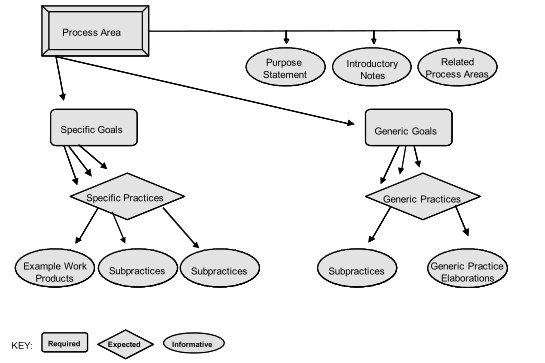
\includegraphics[scale=1]{Images/modelcom.PNG}
	\caption{Componentes de modelo CMMI}
	\label{fig:modelcom}
\end{figure}

\section{Áreas de Proceso}
Ya hemos hablado de los diferentes componentes de los que consta un área de proceso. Recordemos que la definición de lo que es un área de proceso se encuentra en la Sección \ref{sec:terminologia}. Las diferentes áreas de proceso que existen son las siguientes:

\begin{itemize}
	\item Capacity and Availability Management (\textit{CAM})
	\item Causal Analysis and Resolution (\textit{CAR})
	\item Configuration Management (\textit{CM})
	\item Decision Analysis and Resolution (\textit{DAR})
	\item Incident Resolution and Prevention (\textit{IRP})
	\item Integrated Work Management (\textit{IWM})
	\item Measurement and Analysis (\textit{MA})
	\item Organizational Process Definition (\textit{OPD})
	\item Organizational Process Focus (\textit{OPF})
	\item Organizational Performance Management (\textit{OPM})
	\item Organizational Process Performance (\textit{OPP})
	\item Organizational Training (\textit{OT})
	\item Process and Product Quality Assurance (\textit{PPQA})
	\item Quantitative Work Management (\textit{QWM})
	\item Requirements Management (\textit{REQM})
	\item Risk Management (\textit{RSKM})
	\item Supplier Agreement Management (\textit{SAM})
	\item Service Continuity (\textit{SCON})
	\item Service Delivery (\textit{SD})
	\item Service System Development (\textit{SSD})
	\item Service System Transition (\textit{SST})
	\item Strategic Service Management (\textit{STSM})
	\item Work Monitoring and Control (\textit{WMC})
	\item Work Planning (\textit{WP})
\end{itemize}


\section{Representaciones y niveles}
Los niveles surgen como una manera de clasificar cómo se posiciona una organización que quiere mejorar los procesos que emplea para ofrecer sus servicios. Estos procesos se suelen asociar con un área de proceso determinada, de manera que sea posible la evaluación de acuerdo al modelo. El nivel suele ser  resultado de esta evaluación (\textit{appraisal}), que puede llevarse a cabo sobre grupos de trabajo, una división o la organización entera. CMMI soporta dos manera de mejora mediante el uso de niveles:

\begin{itemize}
\item La primera permite la mejora incremental de los procesos que pertenecen a uno o varios áreas de proceso.
\item La segunda permite la mejora de un conjunto de procesos relacionados al abordar incrementalmente conjuntos sucesivos de áreas de proceso.
\end{itemize}

Estas dos vías de mejora se asocian con dos tipos de niveles. A su vez, estos niveles se corresponden con dos aproximaciones de mejora conocidas como \textit{representaciones}. A continuación, se explicarán más en detalle las representaciones, para luego explicar los niveles.

\subsection{Representaciones}
En la Figura \ref{fig:representations} se puede observar la estructura tanto de la representación por fases como de la continua. Se ve que ambas son muy parecidas. La principal diferencia radica en que la representación por fases usa los niveles de madurez para caracterizar el estado en el que se encuentran los procesos de la organización en relación al modelo en su conjunto. Por el contrario, la representación continua usa los niveles de capacidad para caracterizar el estado de los procesos de la organización en relación a un área de proceso individual.

\begin{figure}[h]
	\centering
	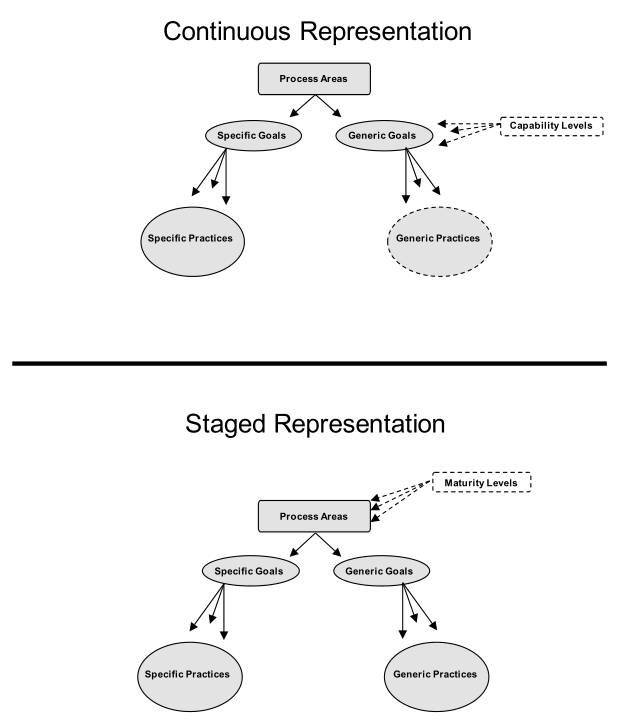
\includegraphics[scale=1]{Images/representations.PNG}
	\caption{Estructura de ambas representaciones}
	\label{fig:representations}
\end{figure}

Así, la representación por fases se preocupa por seleccionar múltiples áreas de proceso para mejorarlas a un nivel de madurez en conjunto. Para la representación por fases, el hecho de que un proceso individual sea realizado o esté incompleto no es relevante. En cambio la representación continua se preocupa por seleccionar tanto el área de proceso que se quiere mejorar como el nivel de capacidad que se quiere alcanzar para ese área de proceso. En este caso, por tanto, el hecho de que un proceso es realizado o incompleto importa.


\subsection{Niveles}
En esta subsección se explicará con mayor detalle los dos tipos de niveles mencionados anteriormente.

\subsubsection{Niveles de capacidad}



\begin{figure}[h]
	\centering
	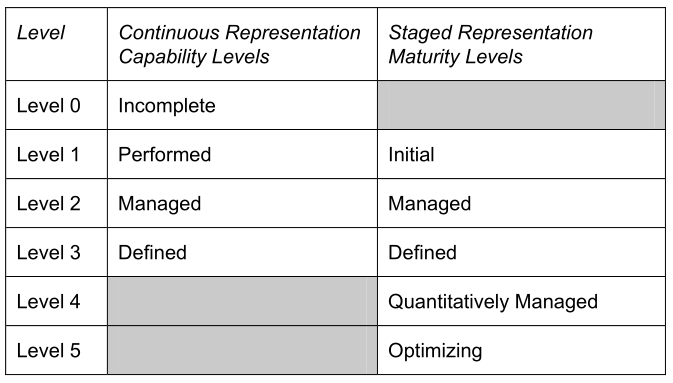
\includegraphics[scale=1]{Images/comparison.PNG}
	\caption{Comparación entre representaciones y niveles}
	\label{fig:comparison}
\end{figure}

		 
\end{itemize}